\clearpage
\section{Pythonによる軌道最適化シミュレーション}
自分でPythonプログラムを書いて、上記手法を実験してみました。実装内容は、ロボットアームモデル・軌道および障害物の可視化関数・目的関数および制約関数・目的関数および制約関数のヤコビアン・scipyを使ったSQP計算になります。

プログラムの実行結果が\figref{figure:2dof}および\figref{figure:5dof}になります。2種類のロボットアームを使って、障害物があるとき/ないときで動作計画しています。補間点数はすべて10点に統一しており、同じロボットアームを使うときは、動作計画開始時の姿勢、終了時のエンドエフェクタ位置を同じにしています。

\figref{figure:2dof}および\figref{figure:5dof}(a)(b)から、障害物回避軌道が生成されていることが確認できます。一方で\figref{figure:5dof}(c)では、障害物を飛び越えるという不本意な軌道が生成されています。\figref{figure:5dof}(b)と障害物の位置が(0.1, 0.1)しかズレていないのに結果が大きく変わってしまい、安定的に収束させることの難しさを実感しました。

今後の課題として考えているのは最適化の初期解の改善です。現在の最適化の初期解はロボットアームの初期姿勢を補間点数分だけ並べたベクトルになっています。本当は軌道最適化計算前にIK計算やRRT計算などを行って、大まかなロボットアーム軌道初期解を複数個は与えるべきだと考えています。

\vspace{-2mm}
\begin{figure}[htbp]
  \begin{minipage}[!h]{0.32\columnwidth}
    \begin{center}
      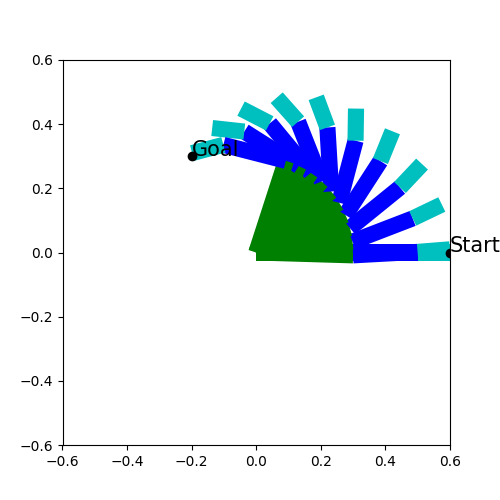
\includegraphics[width=1.0\columnwidth]{figs/2dof_without_obstacle}
      \subcaption{障害物なし。計算時間0.041[s]。}
    \end{center}
  \end{minipage}
  \begin{minipage}[!h]{0.32\columnwidth}
    \begin{center}
      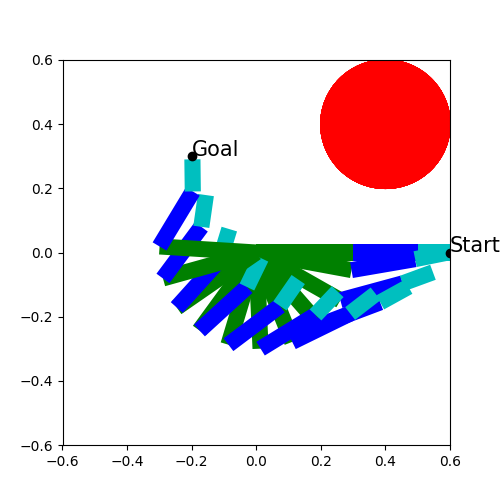
\includegraphics[width=1.0\columnwidth]{figs/2dof_with_obstacle}
      \subcaption{障害物は1個。計算時間0.560[s]。}
    \end{center}
  \end{minipage}
  \caption{2自由度ロボットアームによる障害物回避を考慮した動作計画。カラフルな直方体の連なりがロボットアームで、赤い丸が障害物。}
  \label{figure:2dof}
\end{figure}

\vspace{-8mm}
\begin{figure}[htbp]
  \begin{minipage}[!h]{0.32\columnwidth}
    \begin{center}
      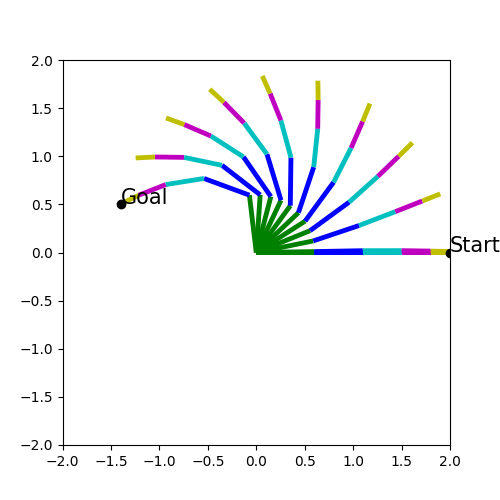
\includegraphics[width=1.0\columnwidth]{figs/5dof_without_obstacle}
      \subcaption{障害物なし。計算時間0.111[s]。}
    \end{center}
  \end{minipage}
  \begin{minipage}[!h]{0.32\columnwidth}
    \begin{center}
      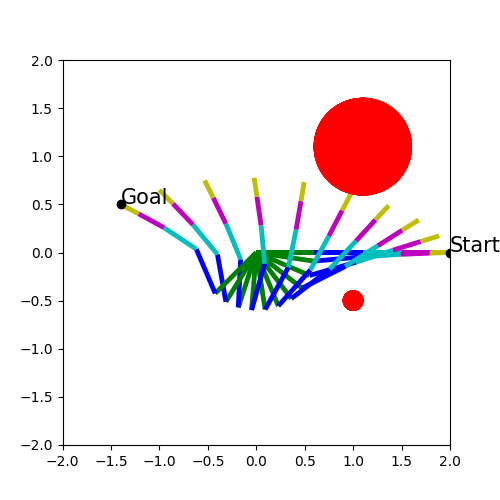
\includegraphics[width=1.0\columnwidth]{figs/5dof_with_obstacle}
      \subcaption{障害物は2個。計算時間5.534[s]。}
    \end{center}
  \end{minipage}
  \begin{minipage}[!h]{0.32\columnwidth}
    \begin{center}
      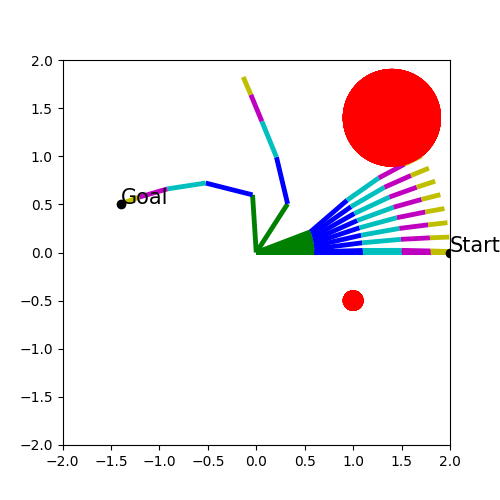
\includegraphics[width=1.0\columnwidth]{figs/5dof_with_obstacle_fail}
      \subcaption{障害物は2個。計算時間5.202[s]。障害物を飛び越える不本意な軌道が生成される。}
    \end{center}
  \end{minipage}
  \caption{5自由度ロボットアームによる障害物回避を考慮した動作計画。カラフルな直方体の連なりがロボットアームで、赤い丸が障害物。}
  \label{figure:5dof}
\end{figure}

最後に、実装したPythonコードを貼ります。また、使用したソフトウェアのバージョンは次のとおりです。Python==2.7.17, numpy==1.16.6, scipy==1.2.1, matplotlib==2.2.5
\\

\fontsize{8pt}{8pt}\selectfont
\begin{verbatim}
#!/usr/bin/env python

import matplotlib.pyplot as plt
import matplotlib.patches as patches
import numpy as np
from scipy.optimize import minimize
import time


class Arm(object):
    """
    This class represents 2D robot arm for collision avoidance
    """

    def __init__(self, link_length):
        """
        self.link_length is a list of link length of robot arm [m]
        self.angle_vector is each joint angle [deg] from root to end effector.
        self.obstacles is list of [x[m], y[m], radius[m]] for obstacle circle
        """
        # Robot config
        self.link_length = link_length
        self.angle_vector = [0.0] * len(link_length)
        # Visualization settings
        self.fig, self.ax = plt.subplots(1, 1, figsize=(5, 5))
        axis_lim = reduce(lambda x, y: x+y, self.link_length)
        self.ax.set_xlim([-axis_lim, axis_lim])
        self.ax.set_ylim([-axis_lim, axis_lim])
        self.colors = ["g", "b", "c", "m", "y", "k", "w"]
        self.viz_links = []
        self.obstacles = []
        self.viz_obstacles = []

    def calc_joints(self):
        """
        Calculate 2D positions of each joints
        """
        joints = np.array([[0, 0]])
        angle_sum = 0
        for i, ll in enumerate(self.link_length):
            angle_sum = angle_sum + self.angle_vector[i]
            link_vec = np.array([ll * np.cos(np.deg2rad(angle_sum)),
                                 ll * np.sin(np.deg2rad(angle_sum))])
            joints = np.append(
                joints,
                np.array([joints[-1] + link_vec]),
                axis=0)
        return joints

    def calc_specific_joints_jac(self, joint_num):
        """
        Calculate 2D jacobian at specific joint coords.
        """
        link_num = len(self.link_length)

        def calc_jac_diff_j(j):
            """
            Calculate 2D jacobian at specific joint coords Differentiated by specific joint
            """
            jac = np.tile(np.array([[0, 0]]), (link_num, 1)).astype(np.float32)
            angle_sum = 0
            for k in range(joint_num):
                angle_sum = angle_sum + self.angle_vector[k]
                if k < j:
                    continue
                ll = self.link_length[k]
                jac[j] = jac[j] + (np.pi / 180.) * np.array([ll * -np.sin(np.deg2rad(angle_sum)),
                                                             ll * np.cos(np.deg2rad(angle_sum))])
            return jac

        ret = np.tile(np.array([[0, 0]]), (link_num, 1)).astype(np.float32)
        for l in range(link_num):
            ret = ret + calc_jac_diff_j(l)
        return ret

    def calc_joints_jac(self):
        """
        Calculate 2D jacobian of each joints
        """
        link_num = len(self.link_length)
        jac = np.tile(np.array([[0, 0]]), (link_num+1, link_num, 1)).astype(np.float32)
        for i in range(link_num+1):
            jac[i] = self.calc_specific_joints_jac(i)
        return jac

    def get_angle_vector(self):
        """
        Get self.angle_vector
        """
        return self.angle_vector

    def set_angle_vector(self, angle_vector):
        """
        Set self.angle_vector by argment
        """
        if len(angle_vector) == len(self.angle_vector):
            self.angle_vector = angle_vector
        else:
            print('angle_vector length should be {}, but {} is given'.format(
                len(self.angle_vector), len(angle_vector)))

    def add_obstacle(self, obstacle_pos):
        """
        Add obstacle to avoid. The obstacle shape must be circle.
        obstacle_pos must be list like [x[m], y[m], radius[m]]
        """
        self.obstacles.append(obstacle_pos)

    def remove_obstacle(self):
        """
        Remove all obstacles to avoid.
        """
        self.obstacles = []

    def get_obstacle(self):
        """
        return all obstacles to avoid.
        """
        return self.obstacles

    def remove_visualize_objects(self):
        for vl in self.viz_links:
            vl.remove()
            self.viz_links = []
        for vo in self.viz_obstacles:
            vo.remove()
            self.viz_obstacles = []

    def visualize(self, remove_previous=True):
        """
        If remove_prevous is True, previous matplotlib patches are removed.
        joints is position of each joint of the robot arm
        height is link thickness
        offset is offset for matplotlib visualization
        """
        # Remove previous plots
        if remove_previous is True:
            self.remove_visualize_objects()
        # Visualize
        joints = self.calc_joints()
        angle_sum = 0
        for i, ll in enumerate(self.link_length):
            angle_sum = angle_sum + self.angle_vector[i]
            link_vec = np.array([ll * np.cos(np.deg2rad(angle_sum)),
                                 ll * np.sin(np.deg2rad(angle_sum))])
            height = 0.05
            offset = np.array([height * np.cos(np.deg2rad(angle_sum+90)) * 0.5,
                               height * np.sin(np.deg2rad(angle_sum+90)) * 0.5])
            rec = patches.Rectangle(
                xy=tuple((joints[i]+joints[i+1])*0.5 - link_vec*0.5 - offset),
                width=ll, height=height, angle=angle_sum,
                fc=self.colors[i])
            self.viz_links.append(rec)
            self.ax.add_patch(rec)
        for i, obs in enumerate(self.obstacles):
            cir = patches.Circle(
                xy=tuple(obs[:2]), radius=obs[2], color='r')
            self.viz_obstacles.append(cir)
            self.ax.add_patch(cir)
        plt.pause(0.1)


class SQP(object):
    """
    Collision avoidance motion planning
    using SQP (Sequential quadratic Programming).
    """

    def __init__(self, arm, target_end_effector_pos, waypoint_num):
        """
        Arguments:
        arm: Arm class instance
        target_end_effector_pos: The last position of end effector
                               This value should be list like [x[m], y[m]]
        waypoint_num: The number of interpolation points.
                      Waypoints means time series trajectory.

        Member variables:
        self.arm_copy: variable for SQP iteration
        self.constraints: A list of constraints functions for SQP
        self.obj_func: Objective function for SQP

        argument in constraint or objective function
        x: waypoints.
           The length is (length of arm angle vector) * (length of waypoints)
        """
        self.last_ee = target_end_effector_pos
        self.waypoint_num = waypoint_num
        self.viz_start_goal = []
        self.set_arm(arm)

    def set_target_end_effector_pos(self, target_end_effector_pos):
        self.last_ee = target_end_effector_pos

    def set_arm(self, arm):
        self.arm_copy = arm
        self.start_ee = self.arm_copy.calc_joints()[-1].tolist()
        self.start_av = self.arm_copy.get_angle_vector()
        self.waypoints = [np.array(self.start_av)]
        self.avl = len(self.arm_copy.get_angle_vector())
        self.constraints = self.constraints_func_and_jac()
        (self.obj_func, self.obj_jac) = self.obj_func_and_jac()

    def constraints_func_and_jac(self):
        # Set constraints functions (Constraints function list for scipy)
        constraints = []
        # 1. obstacle avoidance
        for i in range(self.waypoint_num):
            for j in range(len(self.arm_copy.calc_joints())):
                if j == 0:
                    continue
                for k in self.arm_copy.get_obstacle():
                    def cons(x, waypoint, joint, obstacle):
                        self.arm_copy.set_angle_vector(
                            x[waypoint*self.avl:(waypoint+1)*self.avl])
                        joint_pos = self.arm_copy.calc_joints()[joint]
                        distance = np.linalg.norm(
                            np.array(joint_pos) - np.array(obstacle[:2]))
                        return distance ** 2 - obstacle[2] ** 2
                    def jac(x, waypoint, joint, obstacle):
                        self.arm_copy.set_angle_vector(
                            x[waypoint*self.avl:(waypoint+1)*self.avl])
                        joint_pos = self.arm_copy.calc_joints()[joint]
                        joint_jac = self.arm_copy.calc_joints_jac()[joint]
                        dsdf_dx = 2 * (joint_pos - np.array(obstacle[:2]))
                        ret = np.zeros(len(x))
                        ret[waypoint*self.avl:(waypoint+1)*self.avl] = np.dot(joint_jac, dsdf_dx)
                        return ret
                    constraints.append(
                        {'type': 'ineq', 'fun': cons, 'jac': jac, 'args': (i, j, k)})
        # 2. The last end effector position error must lower than max_error[m]
        max_error = 0.01
        def cons(x):
            self.arm_copy.set_angle_vector(
                x[(self.waypoint_num-1)*self.avl:self.waypoint_num*self.avl])
            joints = self.arm_copy.calc_joints()
            ee_error = np.linalg.norm(
                np.array(joints[-1]) - np.array(self.last_ee))
            return max_error ** 2 - ee_error ** 2
        def jac(x):
            self.arm_copy.set_angle_vector(
                x[(self.waypoint_num-1)*self.avl:self.waypoint_num*self.avl])
            joint_pos = self.arm_copy.calc_joints()[-1]
            joint_jac = self.arm_copy.calc_joints_jac()[-1]
            dsdf_dx = 2 * (np.array(joint_pos) - np.array(self.last_ee))
            ret = np.zeros(len(x))
            ret[(self.waypoint_num-1)*self.avl:self.waypoint_num*self.avl] = np.dot(joint_jac, dsdf_dx)
            return -ret
        constraints.append({'type': 'ineq', 'fun': cons, 'jac': jac})
        # 3. The start end effector position error must lower than max_error[m]
        def cons(x):
            self.arm_copy.set_angle_vector(
                x[0:self.avl])
            joints = self.arm_copy.calc_joints()
            ee_error = np.linalg.norm(
                np.array(joints[-1]) - np.array(self.start_ee))
            return max_error ** 2 - ee_error ** 2
        def jac(x):
            self.arm_copy.set_angle_vector(
                x[0:self.avl])
            joint_pos = self.arm_copy.calc_joints()[-1]
            joint_jac = self.arm_copy.calc_joints_jac()[-1]
            dsdf_dx = 2 * (np.array(joint_pos) - np.array(self.start_ee))
            ret = np.zeros(len(x))
            ret[0:self.avl] = np.dot(joint_jac, dsdf_dx)
            return -ret
        constraints.append({'type': 'ineq', 'fun': cons, 'jac': jac})
        return constraints

    # Set objective function: sum of angle vector velocity
    def obj_func_and_jac(self):
        I_plus = np.identity(self.avl)
        I_minus = np.identity(self.avl) * -1
        I_zeros = np.zeros((self.avl, self.avl))
        A = np.array([], dtype=np.float128)
        for i in range(self.waypoint_num):
            for j in range(self.waypoint_num):
                if j == 0:
                    # initial element for horizontal
                    if i == 0:
                        horizontal = I_plus
                    elif i == 1:
                        horizontal = I_minus
                    else:
                        horizontal = I_zeros
                elif i == j:
                    horizontal = np.append(horizontal, I_plus, axis=1)
                elif i == j + 1:
                    horizontal = np.append(horizontal, I_minus, axis=1)
                else:
                    horizontal = np.append(horizontal, I_zeros, axis=1)
            if len(A) == 0:
                A = horizontal
            else:
                A = np.append(A, horizontal, axis=0)
        B = np.zeros(self.waypoint_num * self.avl)
        B[0:self.avl] = np.array(self.start_av)
        return (lambda x: np.linalg.norm(np.dot(A, x) - B) ** 2,
                lambda x: 2 * np.dot(A.T, np.dot(A, x) - B))

    def make_plan(self):
        """
        Solve SQP and make trajectory with collision avoidance.
        """
        start_time = time.time()
        result = minimize(fun=self.obj_func, jac=self.obj_jac,
                          bounds=[(-720, 720)] * self.avl * self.waypoint_num,
                          x0=self.start_av*self.waypoint_num,
                          constraints=self.constraints, method='SLSQP')
                          # options={"maxiter": 500, "verbose": 2})
        print('t=0: {}'.format(self.start_av))
        self.waypoints = [self.start_av]
        for i in range(self.waypoint_num):
            av = result.x[i*self.avl:(i+1)*self.avl]
            self.waypoints.append(av)
            print('t={}: {}'.format(i+1, av))
        if bool(result.success) is True:  # numpy.bool_ to bool
            print('result: SQP Success')
        else:
            print('result: SQP Fail')
        print('Calculation time: {} [s]'.format(time.time() - start_time))

    def visualize(self, remove_previous=True):
        if len(self.waypoints) == 1:
            print('Plan have not been made yet or SQP is not solved.')
            return
        # Remove previous plots
        self.arm_copy.remove_visualize_objects()
        for v in self.viz_start_goal:
            v.remove()
            self.viz_start_goal = []
        # Start point
        start_dot = self.arm_copy.ax.plot(
            self.start_ee[0], self.start_ee[1], marker="o", color="black")
        start_word = self.arm_copy.ax.text(
            self.start_ee[0], self.start_ee[1], "Start",
            size="15", color="black")
        self.viz_start_goal.append(start_dot[0])
        self.viz_start_goal.append(start_word)
        # Goal point
        goal_dot = self.arm_copy.ax.plot(
            self.last_ee[0], self.last_ee[1], marker="o", color="black")
        goal_word = self.arm_copy.ax.text(
            self.last_ee[0], self.last_ee[1], "Goal",
            size="15", color="black")
        self.viz_start_goal.append(goal_dot[0])
        self.viz_start_goal.append(goal_word)
        # Waypoints
        for waypoint in self.waypoints:
            self.arm_copy.set_angle_vector(waypoint)
            self.arm_copy.visualize(remove_previous=remove_previous)


def sample_arm_rotate():
    arm = Arm([0.3, 0.2, 0.1])
    arm.add_obstacle([0.3, 0.3, 0.1])
    for i in range(30 + 1):
        arm.set_angle_vector([i*12, i*24, i*36])
        arm.visualize()


def sample_sqp():
    # Case 1-1 Normal planning
    arm = Arm([0.3, 0.2, 0.1])
    arm.set_angle_vector([0, 0, 0])
    sqp = SQP(arm, target_end_effector_pos=[-0.2, 0.3], waypoint_num=10)
    sqp.make_plan()
    sqp.visualize(remove_previous=False)

    # Case 1-2 Object avoidance planning
    arm = Arm([0.3, 0.2, 0.1])
    arm.set_angle_vector([0, 0, 0])
    arm.add_obstacle([0.4, 0.4, 0.2])
    sqp = SQP(arm, target_end_effector_pos=[-0.2, 0.3], waypoint_num=10)
    sqp.make_plan()
    sqp.visualize(remove_previous=False)

    # Case 2-1
    arm = Arm([0.6, 0.5, 0.4, 0.3, 0.2])
    arm.set_angle_vector([0, 0, 0, 0, 0])
    sqp = SQP(arm, target_end_effector_pos=[-1.4, 0.5], waypoint_num=10)
    sqp.make_plan()
    sqp.visualize(remove_previous=False)

    # Case 2-2
    arm = Arm([0.6, 0.5, 0.4, 0.3, 0.2])
    arm.set_angle_vector([0, 0, 0, 0, 0])
    arm.add_obstacle([1.1, 1.1, 0.5])
    arm.add_obstacle([1.0, -0.5, 0.1])
    sqp = SQP(arm, target_end_effector_pos=[-1.4, 0.5], waypoint_num=10)
    sqp.make_plan()
    sqp.visualize(remove_previous=False)

    # Case 2-3 (failure)
    arm = Arm([0.6, 0.5, 0.4, 0.3, 0.2])
    arm.set_angle_vector([0, 0, 0, 0, 0])
    arm.add_obstacle([1.2, 1.2, 0.5])
    arm.add_obstacle([1.0, -0.5, 0.1])
    sqp = SQP(arm, target_end_effector_pos=[-1.4, 0.5], waypoint_num=10)
    sqp.make_plan()
    sqp.visualize(remove_previous=False)

    print("Press 'q' to exit")
    plt.show()


if __name__ == '__main__':
    # sample_arm_rotate()
    sample_sqp()
\end{verbatim}
